\documentclass[thesis.tex]{subfiles}

\chapter{Phương pháp sử dụng}

\section{Kiến trúc tổng thể}

Để giải quyết bài toán đặt ra ở phía trên, chúng ta cần phải thực hiện ba giai đoạn khác nhau:
\begin{itemize}
    \item Huấn luyện mô hình phân vùng ảnh ngữ nghĩa trên tập nguồn
    \item Huấn luyện cạnh tranh mô hình trên cả tập nguồn và tập đích (tập đích sử dụng nhãn giả được sinh ra từ mô hình có được từ giai đoạn 1)
    \item Huấn luyện mô hình tự cô đặc bằng nhãn mà nó đã sinh ra ở giai đoạn 2
\end{itemize}

Mô hình tổng quan được xây dựng một cách mềm dẻo với 3 bộ phận khác nhau có thể thay thế và thử nghiệm một cách linh hoạt, bao gồm:
\begin{itemize}
    \item Encoder để trích xuất các đặc trưng của ảnh
    \item Decoder có tác dụng phân loại các điểm ảnh dựa vào thông tin mà Encoder mang lại 
    \item Discriminator phục vụ cho giai đoạn huấn luyện cạnh tranh nhằm học các thông tin từ ảnh không nhãn (miền đích)
\end{itemize}

Luồng kết hợp của bài toán được thể hiện như hình \ref{fig:proposal_overview}. 
\begin{figure}[htp]
	\centering
	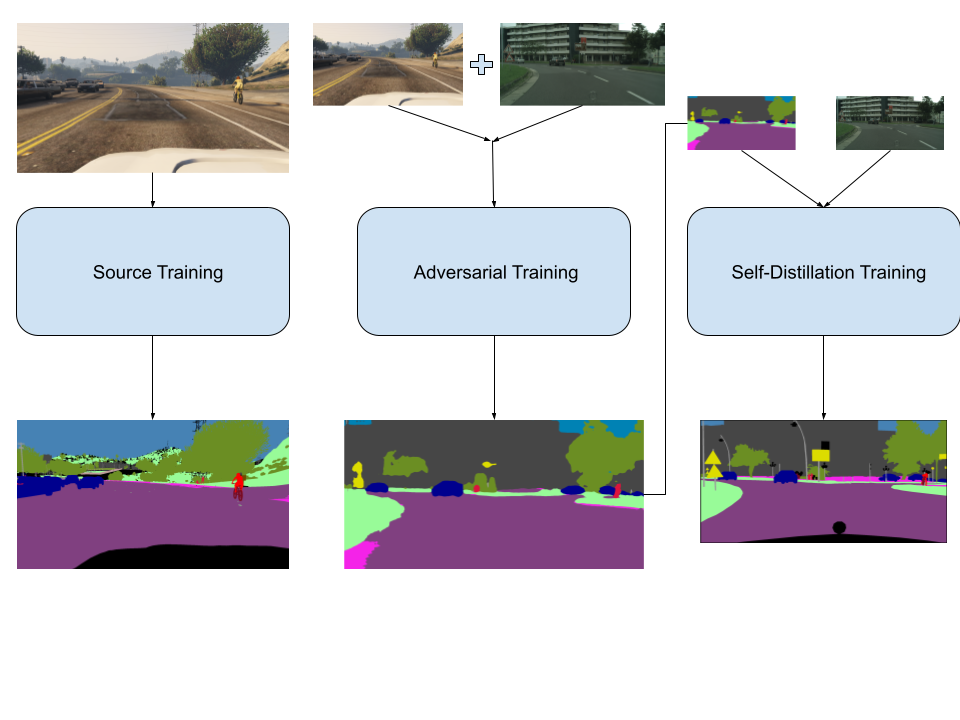
\includegraphics[width=0.8\textwidth]{images/proposal_overview.png}
	\caption{Kiến trúc tổng thế của mô hình\protect\footnotemark}
	\label{fig:proposal_overview}
\end{figure}
\FloatBarrier

\section{Bộ trích xuất đặc trưng}
Mô hình thử nghiệm với 2 kiến trúc Encoder khác nhau là Resnet101 và Hardnet68 

\subsubsection{Resnet} 
Mạng Resnet \cite{he2016deep} được sinh ra nhằm mục đích giúp cho mô hình học sâu hơn nhưng không bị biến mất đạo hàm (vanishing gradient). Đây là hiện tượng Gradient thường sẽ có giá trị nhỏ dần khi đi xuống các layer thấp hơn. Dẫn đến kết quả là các cập nhật thực hiện bởi Gradients Descent không làm thay đổi nhiều trọng số của các tầng đó và làm chúng không thể hội tụ và mạng sẽ không thu được kết quả tốt. Mạng Resnet có thể làm được điều này là nhờ vào khối phần dư. Trong đó, đầu vào $x$ được thêm trực tiếp vào khối phần dư của mạng trở thành $F(x) + x$ được gọi là kết nối bỏ qua (skip connection) hoặc kết nối tắt.

\begin{figure}[htp]
	\centering
	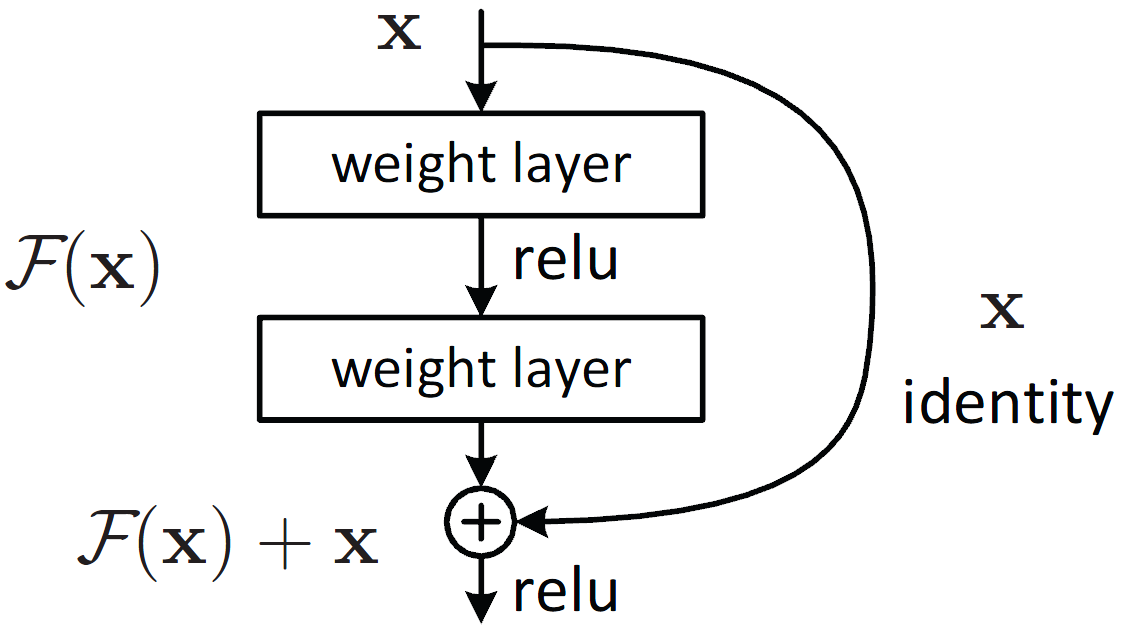
\includegraphics[width=0.6\textwidth]{images/resnet.png}
	\caption{Kiến trúc kết nối bỏ qua của Resnet\protect\footnotemark}
	\label{fig:proposal_overview}
\end{figure}
\FloatBarrier

Có 2 kiến trúc khối trong Resnet đó là \hl{\textbf{Khối cơ bản}} và \hl{\textbf{Khối cổ chai}} thể hiện trong Hình \ref{fig:bottleneck}:
\begin{itemize}
    \item \hl{\textbf{Khối cơ bản}} thường được sử dụng trong các mạng không quá sâu. Sử dụng 2 lớp tích chập 3x3.
    \item \hl{\textbf{Khối cổ chai}} thường được sử dụng cho các mạng có kiến trúc sâu hơn. Đầu tiên sử dụng tích chập 1x1 để giảm kích thước, sau đó tích chập 3x3 và cuối cùng sử dụng kích thước 1x1 để khôi phục kích thước ban đầu.
\end{itemize}

\begin{figure}[htp]
	\centering
	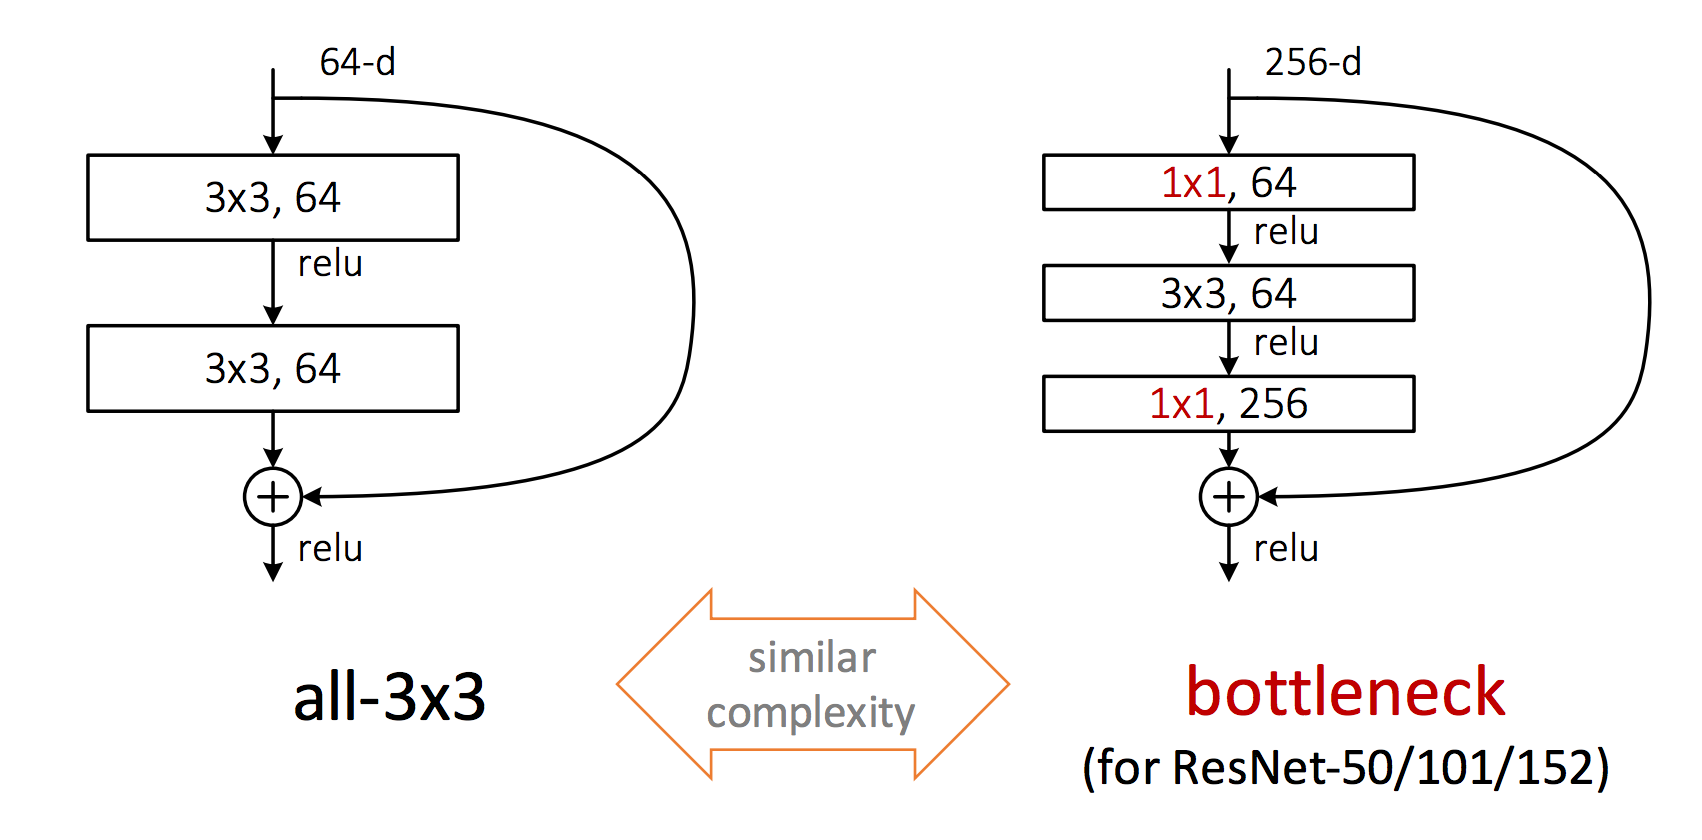
\includegraphics[width=0.6\textwidth]{images/bottleneck.png}
	\caption{Kiến trúc khối cơ bản và khối cổ chai trong Resnet\protect\footnotemark}
	\label{fig:bottleneck}
\end{figure}
\FloatBarrier

\subsubsection{HarDnet} 

Hardnet \cite{chao2019hardnet} được lấy cảm hứng từ Densenet\cite{huang2017densely}. Densenet khá tương đồng với Resnet nhưng kiến trúc gồm các lớp chuyển tiếp và các khối dày đặc. Khối dày đặc này tương tự như khối phần dư tuy nhiên kiến trúc không sử dụng phép cộng mà sử dụng phép ghép nối. Điều này khiến cho mô hình trở nên nặng hơn. Lớp chuyển tiếp được cấu tạo bằng cách kết hợp một lớp tích chập làm giảm độ sâu và một lớp maxpooling làm giảm kích thước nhằm giảm chiều dữ liệu. So sánh Khối phần dư và Khối dày đặc trong Hình \ref{fig:resvsdense}

\begin{figure}[htp]
	\centering
	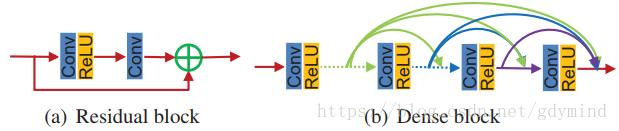
\includegraphics[width=0.6\textwidth]{images/resvsdense.png}
	\caption{Kiến trúc khối phần dư và khối dày đặc\protect\footnotemark}
	\label{fig:resvsdense}
\end{figure}
\FloatBarrier

Không giống như sự thưa thớt được đề xuất trong LogDenseNet\cite{hu2017log}, chúng tôi để tầng $k$ kết nối với tầng $k-2^{n}$ nếu $2^{n}$ chia hết cho $k$, với n là số nguyên không âm và $k-2^{n} \geq 0$; cụ thể, lớp 0 là lớp đầu vào. Dưới lược đồ kết nối này (Hình \ref{fig:hardnet}), một khi lớp $2^{n}$ được xử lý, lớp $1$ đến $2^{n} – 1$ có thể được xóa khỏi bộ nhớ. Các kết nối làm cho mạng xuất hiện dưới dạng chồng chéo của sóng hài bậc hai. Do đó nó có tên là Harmonic Density Connected (HarDNet). Đề án phân biệt hóa được đề xuất giảm chi phí nối tốt hơn đáng kể so với LogDenseNet thuần. Kiểu kết nối này cũng giống như một FractalNet\cite{larsson2016fractalnet} , ngoại trừ cái sau sử dụng các phím tắt tính trung bình thay vì nối.

\begin{figure}[htp]
	\centering
	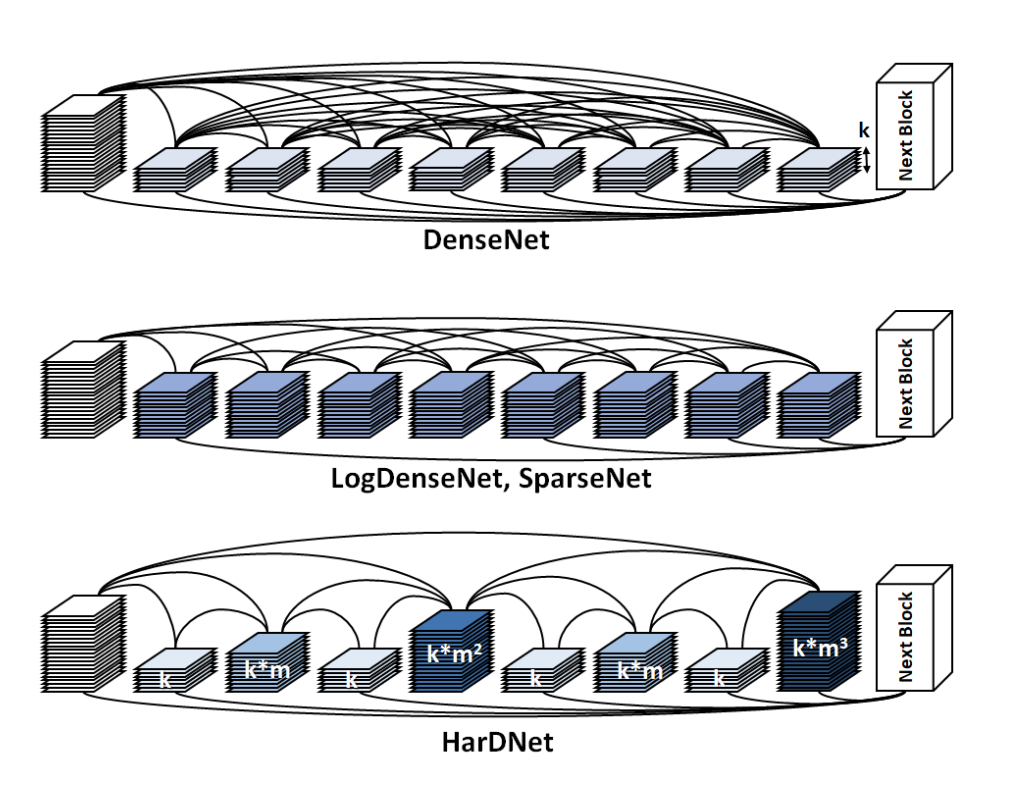
\includegraphics[width=0.6\textwidth]{images/hardnet.png}
	\caption{Hình minh họa cho DenseNet, LogDenseNet, SparseNet và Harmonic DenseNet được đề xuất (HarDNet), trong đó mỗi lớp là một tích chập 3x3\protect\footnotemark}
	\label{fig:hardnet}
\end{figure}
\FloatBarrier

% \begin{minipage}{\linewidth}
% \begin{lstlisting}[caption={An example UserModel wrapped around a simple CNN}]
% import torch
% import torch.nn as nn
% import torch.nn.functional as F

% class Net(nn.Module):
% # ConvNet with 2 convolution blocks followed by dropout 
% # and 2 fully connected layers
%     def __init__(self):
%         super(Net, self).__init__()
%         self.conv1 = nn.Conv2d(1, 10, kernel_size=5)
%         self.conv2 = nn.Conv2d(10, 20, kernel_size=5)
%         self.conv2_drop = nn.Dropout2d()
%         self.fc1 = nn.Linear(320, 50)
%         self.fc2 = nn.Linear(50, 10)

%     def forward(self, x):
%         x = F.relu(F.max_pool2d(self.conv1(x), 2))
%         x = F.relu(F.max_pool2d(self.conv2_drop(self.conv2(x)), 2))
%         x = x.view(-1, 320)
%         x = F.relu(self.fc1(x))
%         x = F.dropout(x, training=self.training)
%         x = self.fc2(x)
%         return x

% class UserModel(Net):
%     def loss(self, output, target):
%         return F.cross_entropy(output, target, reduction='mean')

%     def metrics(self, output, target):
%         preds = torch.argmax(output, dim=1)
%         total = preds.shape[-1]
%         correct = (preds == target).float()
%         acc = torch.sum(correct) / total
%         return {
%             'accuracy': acc.item()
%         }
% \end{lstlisting}
% \end{minipage}



\section{Bộ giải mã}

\subsubsection{Atrous Spatial Pyramid Pooling} 

Atrous Spatial Pyramid Pooling \cite{chen2017deeplab} hay \gls{aspp} là một loại tích chập để phân vùng mạnh mẽ các đối tượng ở nhiều kích thước bằng các bộ lọc ở nhiều tỷ lệ lấy mẫu và trường xem hiệu quả khác nhau. Ưu điểm của \gls{aspp} là không làm giảm chiều của bản đồ đặc trưng quá sâu nhưng vẫn giữ số lượng tham số và chi phí tính toán tương đương mạng nơ-ron tích chập. 

Dữ liệu đầu vào (đầu ra của bộ trích xuất đặc trưng) sẽ được đưa qua đồng thời 4 mạng nơ-ron tích chập với bộ lọc 3x3 và các tham số khác như padding và dilation. Điều này giúp một Atrous convolution với tỷ lệ R thêm các số không R-1 giữa giá trị liên tục để nó phóng to bộ lọc k-kernel thành K + (K-1) (R-1) mà không tăng số lượng tham số. Kết quả được tổng hợp bằng cách cộng các kết quả từ cả 4 mạng lại với nhau, như trong hình \ref{fig:aspp-rate}

\begin{figure}[htp]
	\centering
	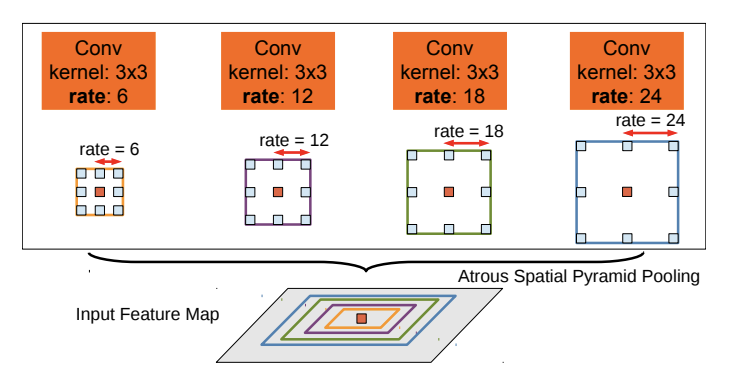
\includegraphics[width=0.6\textwidth]{images/aspp-rate.png}
	\caption{Để phân loại các điểm ảnh trung tâm (màu cam), \gls{aspp} khai thác đặc trưng đa kích thước bằng cách sử dụng nhiều bộ lọc song song với các tỷ lệ khác nhau. Trường nhìn hiệu quả được hiển thị bằng các màu khác nhau\protect\footnotemark}
	\label{fig:aspp-rate}
\end{figure}
\FloatBarrier

\subsubsection{\gls{gald}} 

Tác giả thử cải tiến bằng cách sử dụng một kiến trúc cơ sở do nhóm đề xuất cho giai đoạn 1 nhằm khớp dữ liệu nguồn một cách tốt hơn. 

\begin{figure}[htp]
	\centering
	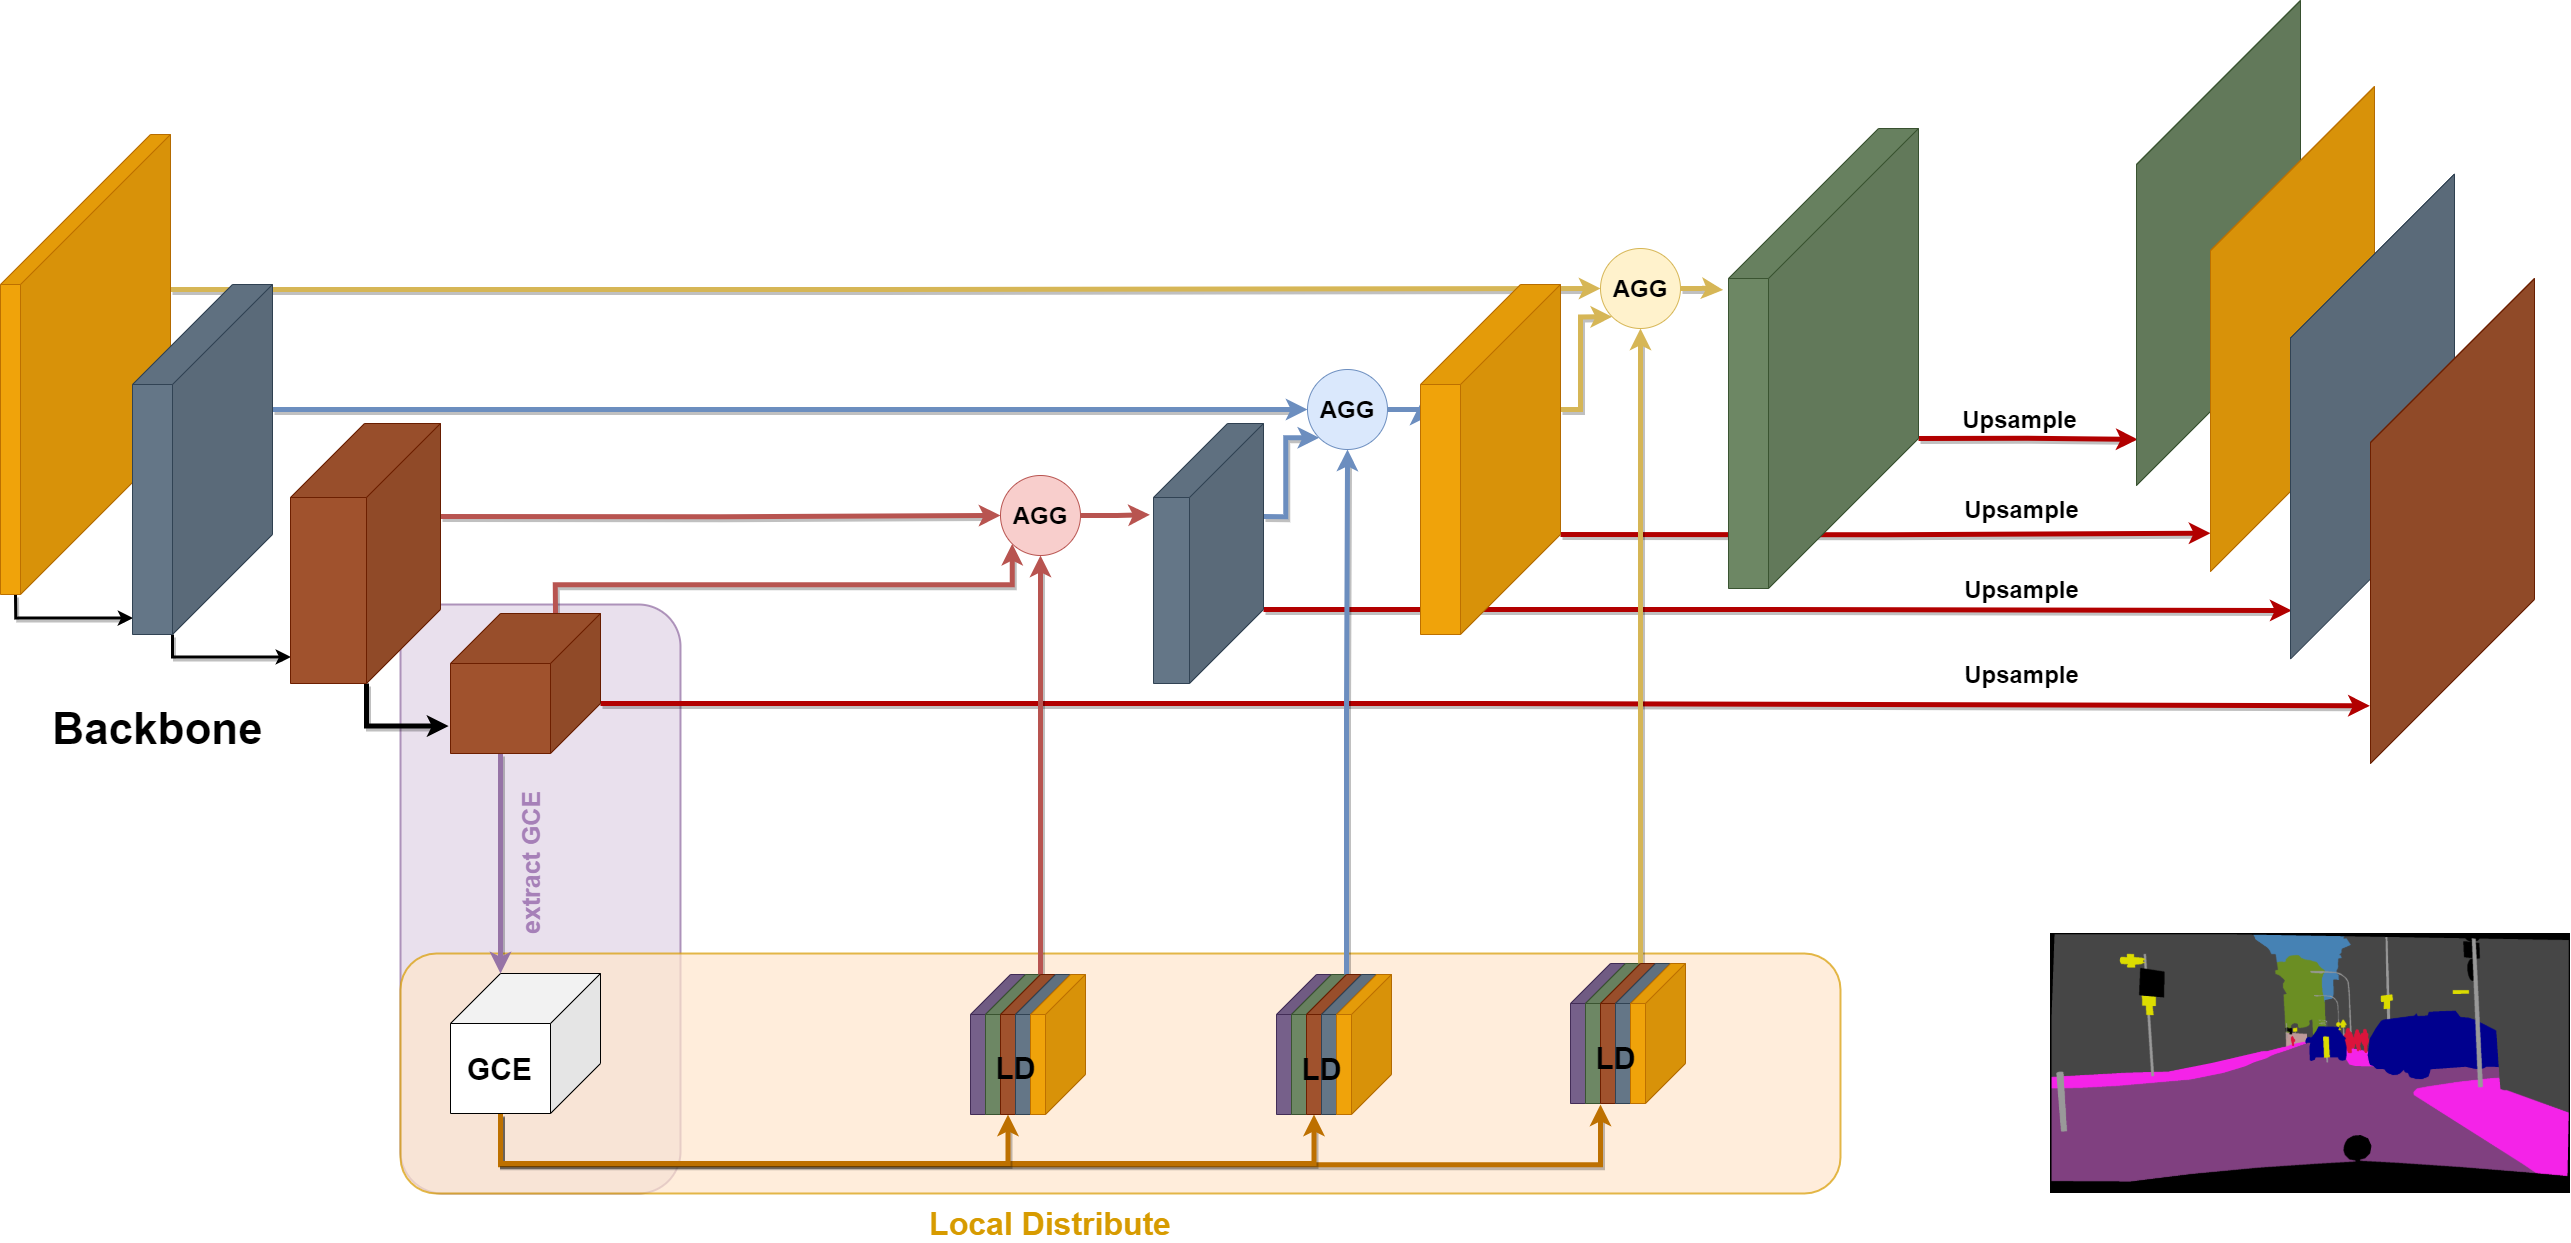
\includegraphics[width=0.6\textwidth]{images/gald.png}
	\caption{Kiến trúc Hardnet68 được kết hợp với GALD để tăng khả năng khớp dữ liệu của mô hình \protect\footnotemark}
	\label{fig:gald}
\end{figure}
\FloatBarrier

Mô hình tổng quan (Hình \ref{fig:gald}) được xây dựng như một biến thể của mạng Unet \cite{ronneberger2015u}. Ảnh đường phố đầu tiên sẽ được đưa qua các mô hình cơ sở để trích xuất đặc trưng và thu được các thông tin bậc cao. Qua mỗi lớp gồm một tập các khối convolution và pooling, độ phân giải của ảnh sẽ bị giảm một nửa tuy nhiên số kênh sẽ tăng lên gấp đôi do đó đặc trưng sẽ có ít thông tin về không gian (góc, cạnh,... ) thay vào đó là thông tin về ngữ nghĩa. Đặc trưng ở lớp cuối cùng sẽ được đi qua lớp global context encoder(GCE) để lấy được thông tin ngữ cảnh và sau đó phân phối lại các đối tượng cụ thể bằng local distribution(LD). Cuối cùng, mô hình sử dụng một lớp Aggregator(AGG) để kết hợp các thông tin bậc cao, bậc thấp và toàn cục để đưa dần ảnh về độ phân giải ban đầu để đưa qua lớp phân loại.


\section{Học đối nghịch}

\subsection{Tổng quan về mạng GAN}

Khi nhắc đến học đối nghịch, ta không thể không đề cập đến kiến trúc mạng GAN (Generative Adversarial Network) \cite{creswell2018generative}. GAN thuộc họ các mô hình sinh dữ liệu. Các mô hình sinh có thể tạo ra các đầu ra có ý nghĩa mới được cung cấp các mã hóa tùy ý. Ví dụ: GAN có thể tạo khuôn mặt người nổi tiếng mới không phải là người thật bằng cách thực hiện phép nội suy không gian tiềm ẩn. Ta có thể áp dụng hiệu quả ý tưởng này cho những bộ dữ liệu không gán nhãn hay nói đúng hơn là việc gán nhãn rất tốn kém chi phí và thời gian.

Mô hình tổng quát của mạng GAN bao gồm 2 bộ phận là bộ sinh (generator) và bộ phân biệt (discriminator) có vai trò tương tự như một kẻ làm giả và một cảnh sát. Mục tiêu của kẻ làm giả là tạo ra những tờ tiền giả nhằm đánh lừa cảnh sát. Ngược lại, nhiệm vụ của cảnh sát là phân biệt được đâu là tiền giả và đâu là tiền thật.  

\begin{figure}[htp]
	\centering
	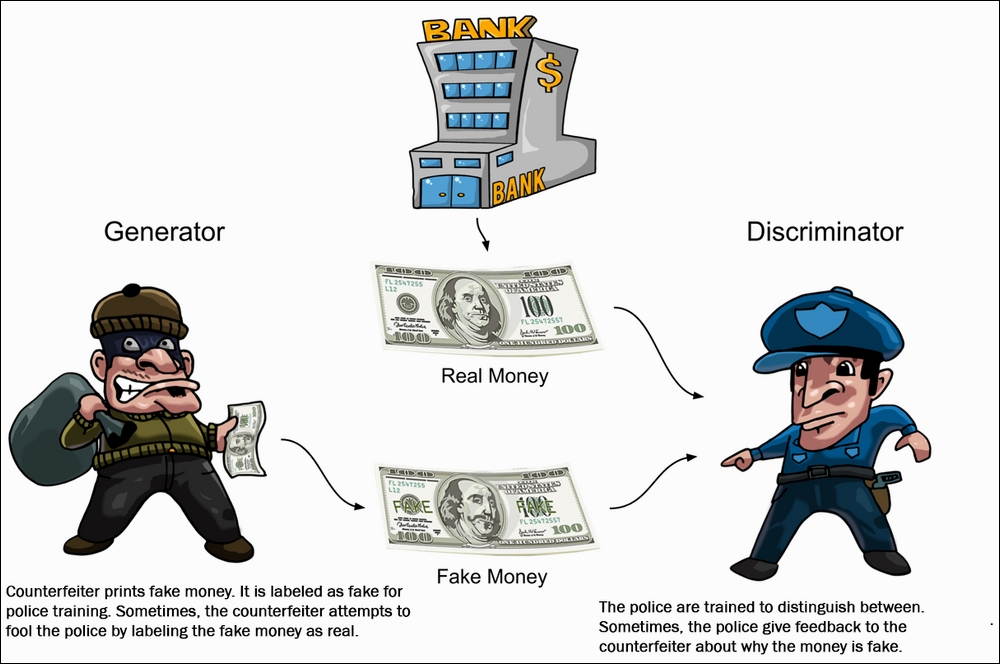
\includegraphics[width=0.6\textwidth]{images/gan_structure.jpeg}
	\caption{Kiến trúc tổng quát của mạng GAN được minh hoạ như sự cạnh tranh giữa kẻ làm tiền giả và cảnh sát\protect\footnotemark}
	\label{fig:proposal_overview}
\end{figure}
\FloatBarrier

Áp dụng ý tưởng đó vào bài toán thích ứng miền cho ảnh đường phố, ta có thể sử dụng thêm bộ phân biệt có nhiệm vụ phân biệt ảnh thuộc miền nguồn hay miền đích. Trong khi đó, bộ trích xuât đặc trưng (Encoder) được coi như một generator có nhiệm vụ trích xuất ra các thông tin từ ảnh của cả 2 miền sao cho có thể đánh lừa được bộ phân biệt. Để làm tốt nhiệm vụ này, việc lựa chọn hàm mất mát phù hợp là rất quan trọng. 

\subsection{Hàm mất mát sử dụng}

Trong suốt quá trình huấn luyện, bộ phân biệt không chỉ có nhiệm vụ phân biệt xem ảnh nào thuộc miền nào, mà còn có vai trò học các cấu trúc lớp của mô hình, hay nói các khác là phân biệt ảnh đầu vào đến mức lớp, xem ảnh nào thuộc miền nào và điểm ảnh thuộc lớp nào. 

$$
\mathcal{L}_{D}=-\sum_{i=1}^{n_{s}} \sum_{k=1}^{K} a_{i k}^{(s)} \log P\left(d=0, c=k \mid f_{i}\right)-\sum_{j=1}^{n_{t}} \sum_{k=1}^{K} a_{j k}^{(t)} \log P\left(d=1, c=k \mid f_{j}\right)
$$

Đặc trưng của hàm GAN chính là ở hàm mất mát cạnh tranh. Hàm mất mát cạnh tranh $\mathcal{L}_{a d v}$ được dùng nhằm đánh lừa bộ phân biệt.
$\mathcal{L}_{a d v}$ được thiết kế để tối đa hoá xác suất của các đặc trưng từ miền đích được coi như là các đặc trưng nguồn mà không phá hỏng đi mối quan hệ giữa các đặc trưng và các lớp. 

$$
\mathcal{L}_{a d v}=-\sum_{j=1}^{n_{t}} \sum_{k=1}^{K} a_{j k}^{(t)} \log P\left(d=0, c=k \mid f_{j}\right)
$$

\subsection{Kiến trúc bộ phân biệt}
Để làm cho bộ phân biệt không chỉ tập trung vào việc phân biệt các miền, ta chia mỗi kênh trong số hai kênh đầu ra của bộ phân biệt nhị phân thành $K$ (số lớp cần phân loại) kênh và khuyến khích việc học cạnh tranh ở mức độ chi tiết.

Để minh họa các chiến lược khác nhau tạo mã hóa cho các miền. Ở đây ta so sánh ba chiến lược khác nhau để trích xuất kiến thức từ mạng phân đoạn để xây dựng mã hóa miền: nhãn miền nhị phân, nhãn cứng 0 1 và nhãn mềm đa kênh. Hình \ref{fig:softhardlabel}

\begin{figure}[htp]
	\centering
	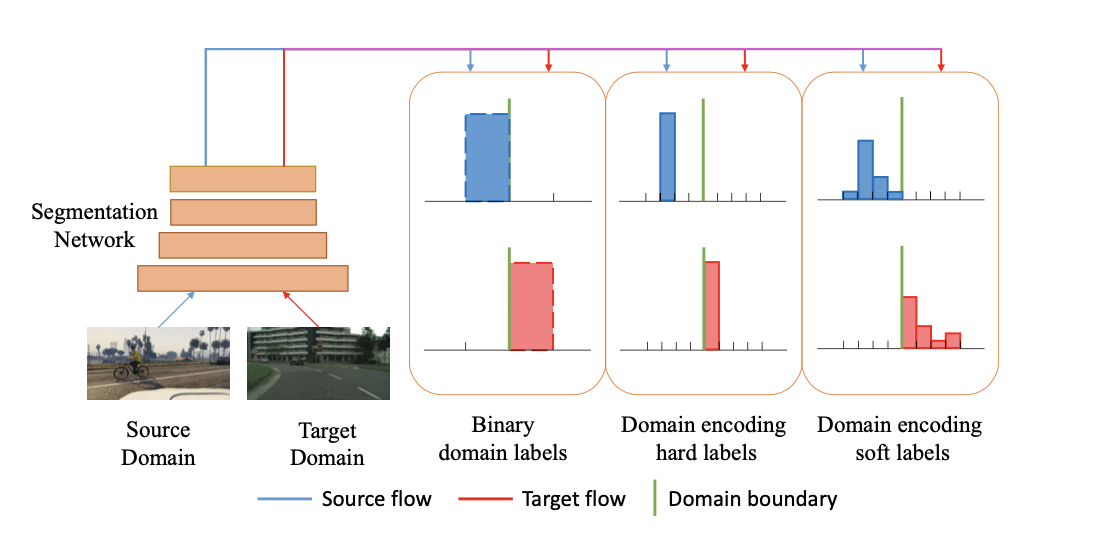
\includegraphics[width=0.6\textwidth]{images/softhardlabel.png}
	\caption{Từ trái sang phải lần lượt là nhãn nhị phân, nhãn cứng với chỉ số 0 1, nhãn mềm\protect\footnotemark}
	\label{fig:softhardlabel}
\end{figure}
\FloatBarrier

Ta sử dụng bộ phân biệt với kiến trúc như sau:
Đối với bộ phân biệt chi tiết, ta áp dụng một cấu trúc đơn giản bao gồm 3 lớp tích chập với số kênh {256, 128, 2$K$}, bộ lọc 3 × 3 và độ dịch chuyển là 1. Mỗi lớp tích chập được theo sau bởi một hàm Leaky-ReLU được tham số hóa bởi 0,2 ngoại trừ lớp cuối cùng. Hình \ref{fig:discriminator}

\begin{figure}[htp]
	\centering
	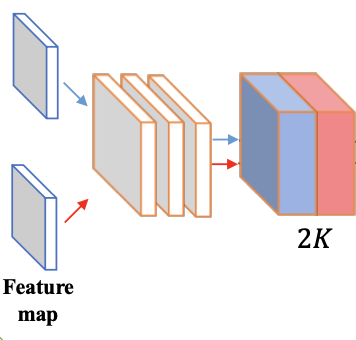
\includegraphics[width=0.4\textwidth]{images/discriminator.png}
	\caption{Bộ phân biệt có tác dụng nhằm giúp cho bộ mã hoá căn chỉnh các đặc trưng của 2 miền ảnh nhằm tìm ra những điểm chung nhất giữa 2 miền\protect\footnotemark}
	\label{fig:discriminator}
\end{figure}
\FloatBarrier

\section{Học chắt lọc}

\subsection{Chắt lọc kiến thức}
Để giải quyết độ trễ, độ chính xác và nhu cầu tính toán tại thời điểm sử dụng mô hình phân loại, chúng ta có thể sử dụng kỹ thuật nén mô hình:
\begin{itemize}
    \item Lượng tử hóa mô hình, số học có độ chính xác thấp để suy luận, ví dụ như chuyển đổi một số thực sang một số nguyên không dấu
    \item Cắt tỉa, loại bỏ trọng số hoặc các hàm kích hoạt gần bằng 0 để thu nhỏ mô hình hơn
    \item Chắt lọc kiến thức: một mô hình phức hợp lớn chắt lọc kiến thức của nó và chuyển hoá nó để đào tạo một mạng lưới nhỏ hơn. Mạng nhỏ hơn cố gắng khớp với các dự đoán và phân phối của mạng lớn hơn
\end{itemize}

Mạng "giáo viên" và "học sinh" thường có các đặc điểm sau đây:
\begin{itemize}
    \item Giáo viên: Mô mình lớn hoặc là tập hợp của các mô hình (khá nhiều tham số cồng kềnh)
    \item Học sinh: thường nhỏ và gọn nhẹ
\end{itemize}

Chắt lọc kiến thức nghĩa là đào tạo mạng học sinh bằng cách sử dụng kiến thức chắt lọc được ngoại suy từ mạng giáo viên, học sinh cố gắng hết sức để tiếp thu mọi thứ do giáo viên giảng dạy (mô hình học sinh được đào tạo để khái quát hóa theo cùng một cách với giáo viên). Một mô hình nhỏ được đào tạo để tổng quát hóa theo cùng một cách thường sẽ làm tốt hơn nhiều trên dữ liệu thử nghiệm so với một mô hình nhỏ được đào tạo theo cách thông thường trên cùng một tập hợp đào tạo đã được sử dụng để đào tạo nhóm. Lưu ý là mô hình lớn nên đạt được hiệu suất \gls{sota}. Ta có thể hình dung các hoạt động của phương pháp này như hình \ref{fig:proposal_overview}

\begin{figure}[htp]
	\centering
	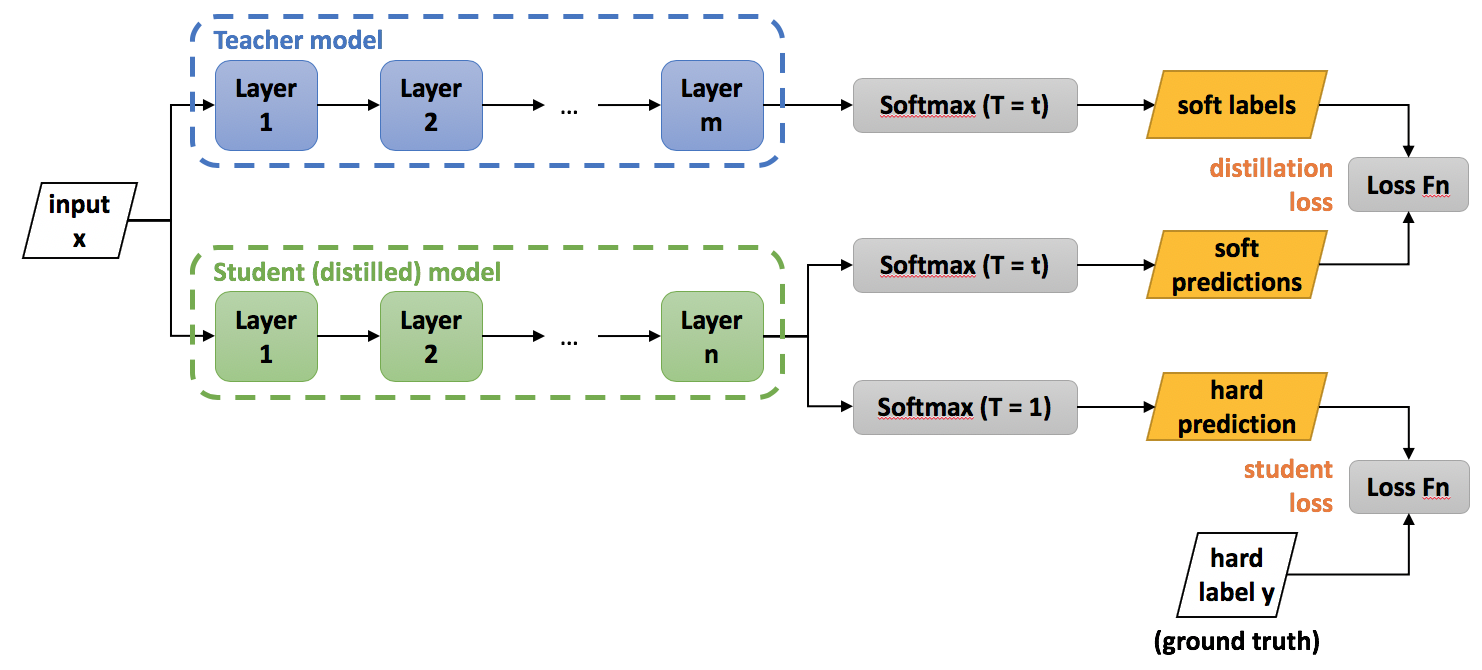
\includegraphics[width=0.6\textwidth]{images/knowledge_distillation.png}
	\caption{Mô hình tổng quát của học cô đọng kiến thức\protect\footnotemark}
	\label{fig:knowledge_distillation}
\end{figure}
\FloatBarrier

\subsection{Tự chắt lọc}
Trong bài toán này ta sẽ áp dụng phép tự chắt lọc. Ở đó, mô hình giáo viên và mô hình học sinh có cấu trúc không khác gì nhau. Ta sẽ sử dụng các xác suất lớp được suy ra từ mô hình lớn như là các "nhãn mềm" cho việc huấn luyện mô hình nhỏ. Công thức cụ thể như sau: 

$$
q_{i}=\frac{\exp \left(z_{i} / T\right)}{\sum_{j} \exp \left(z_{j} / T\right)}
$$

Trong đó $T$ là nhiệt độ, sử dụng giá trị $T$ lớn có thể xuất ra một phân phối xác suất mềm hơn trên tất cả các lớp. Để giải thích cho điều này, ta nhận thấy rằng với mỗi điểm ảnh đã được dự đoán, nếu giữ nguyên xác suất được tính ra từ mô hình hoặc sử dụng "nhãn cứng" 0 1 thì khi đó thông tin về các nhãn sai sẽ bị giảm đi vai trò hay thậm chí là không có vai trò gì. 

\begin{figure}[htp]
	\centering
	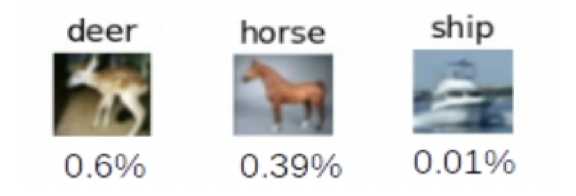
\includegraphics[width=0.4\textwidth]{images/temperature.png}
	\caption{"Nhãn mềm" linh hoạt và cung cấp nhiều thông tin hơn "nhãn cứng"\protect\footnotemark}
	\label{fig:knowledge_distillation}
\end{figure}
\FloatBarrier

"Nhãn mềm" với giá trị $T$ sẽ chứa thông tin có giá trị dữ liệu phong phú hơn. Cung cấp nhiều thông tin hơn và ít chênh lệch hơn về gradient trong quá trình huấn luyện. Cho phép mô hình học sinh nhỏ hơn được huấn luyện trên dữ liệu nhỏ hơn nhiều so với mô hình cồng kềnh ban đầu và với tốc độ học tập cao hơn nhiều.